\documentclass{article} % For LaTeX2e
\usepackage{iclr2017_conference,times}
\usepackage{hyperref}
\usepackage{url}



\usepackage{amsmath,graphicx}
\usepackage{algorithm}
\usepackage[noend]{algpseudocode}

\makeatletter
\def\BState{\State\hskip-\ALG@thistlm}
\makeatother


%\usepackage[cmex10]{amsmath}
\usepackage{amssymb}
\usepackage{amsthm}
\usepackage{geometry}
\usepackage{graphicx}
\usepackage{epstopdf}
\usepackage{hyperref}
% \usepackage[francais]{babel}
\usepackage[applemac]{inputenc}
\usepackage{color}

%\usepackage{graphicx}% Include figure files
%\usepackage{dcolumn}% Align table columns on decimal point
%\usepackage{bm}% bold math
%\usepackage{color}
%\usepackage[caption=false]{subfig} 

\usepackage{listings}

\definecolor{dkgreen}{rgb}{0,0.6,0}
\definecolor{gray}{rgb}{0.5,0.5,0.5}
\definecolor{mauve}{rgb}{0.58,0,0.82}

\lstset{frame=tb,
  language=python,
  aboveskip=3mm,
  belowskip=3mm,
  showstringspaces=false,
  columns=flexible,
  basicstyle={\small\ttfamily},
  numbers=none,
  numberstyle=\tiny\color{gray},
  keywordstyle=\color{blue},
  commentstyle=\color{dkgreen},
  stringstyle=\color{mauve},
  breaklines=true,
  breakatwhitespace=true,
  tabsize=3
}

\newcommand {\lb} {{\langle}}
\newcommand {\rb} {{\rangle}}
\newcommand {\R} {{\mathbb{R}}}
\newcommand {\X} {{\tilde X}}
\newcommand {\w} {{\tilde w}}
\newcommand {\hh} {{k}}
\newcommand {\p} {{\tilde p}}
\newcommand {\RN} {{{\mathbb{R}}^N}}
\newcommand {\Z} {{\mathbb{Z}}}
\newcommand {\E} {{\mathbb{E}}}
\newcommand {\W} {{\cal{W}}}
\newcommand {\Fem} {F_{e}}
\newcommand {\Forr} {F_{o}}
\newcommand{\Exp}[1]{\mathbb{E}\left(#1 \right)}

\usepackage{amsthm}
\usepackage{amsmath}
\usepackage{amssymb}


\newcommand{\figref}[1]{Fig. \ref{#1}}


\newtheorem{theorem}{Theorem}[section]
\newtheorem{lemma}[theorem]{Lemma}
\newtheorem{proposition}[theorem]{Proposition}
\newtheorem{corollary}[theorem]{Corollary}


\title{Topology and Geometry of Deep Rectified Network Optimization Landscapes }


\author{C. Daniel Freeman \thanks{ See our github page at PAGEGOHERE} \\
Department of Physics\\
University of California at Berkeley\\
Berkeley, CA 94720, USA \\
\texttt{daniel.freeman@berkeley.edu} \\
\And
Joan Bruna \\
Courant Institute of Mathematical Sciences \\
New York University \\
New York, NY 10011, USA \\
\texttt{bruna@cims.nyu.edu} \\
}

% The \author macro works with any number of authors. There are two commands
% used to separate the names and addresses of multiple authors: \And and \AND.
%
% Using \And between authors leaves it to \LaTeX{} to determine where to break
% the lines. Using \AND forces a linebreak at that point. So, if \LaTeX{}
% puts 3 of 4 authors names on the first line, and the last on the second
% line, try using \AND instead of \And before the third author name.

\newcommand{\fix}{\marginpar{FIX}}
\newcommand{\new}{\marginpar{NEW}}

%\iclrfinalcopy % Uncomment for camera-ready version

\begin{document}


\maketitle

\begin{abstract}
The loss surface of deep neural networks has recently attracted interest 
in the optimization and machine learning communities as a prime example of 
high-dimensional non-convex problem. Some insights were recently gained using spin glass 
models, but at the expense of strongly simplifying the nonlinear nature of the model.

In this work, we do not make any such assumption and study conditions 
on the data distribution and model architecture that prevent the existence 
of bad local minima. Our theoretical work quantifies and formalizes two 
important qualitative facts: (i) the landscape of deep linear networks is radically different 
from that of deep half-rectified ones, thus implying that mean-field approximations
are unable to capture essential nonlinear behavior, and (ii) that the energy landscape 
in the non-linear case is fundamentally controlled by the interplay between the smoothness of the data distribution and model over-parametrization. 
These results are in accordance with empirical practice and recent literature. 
%Together with 
%recent results that rigorously establish that no gradient descent can 
%get stuck on saddle points, we conclude that gradient descent converges
%to a global optimum in deep rectified networks. 

The conditioning of gradient descent is the next challenge we address. 
We study this question by estimating the geometry of level sets, and we introduce
an algorithm to estimate the regularity of such sets on large-scale networks. 
Our empirical results show that these level sets remain connected throughout 
all the learning phase, but they become exponentially more curvy 
as the energy level decays, in accordance to what is observed in practice with 
very low curvature attractors.
\end{abstract}

%\tableofcontents

%%%%%%%%%%%%%%%%%%%%%%
%%%%%%%%%%%%%%%%%%%%%%
\section{Introduction}
\label{sec:Intro}
%%%%%%%%%%%%%%%%%%%%%%

\begin{itemize}
\item Context of the problem
\item Related work: Spin glass, recent results from Shamir. Gradient Descent converges to minimizers (Jordan Recht et al). 
\item Topology of the level sets. Main result on connectedness of level sets.
\item Geometry of the level sets. Algorithm to estimate the geodesics along level sets. Measure of curvature of these sets. 
\end{itemize}
  


\section{Topology of Level Sets}

Let $P$ be a probability measure on a product space $\mathcal{X} \times \mathcal{Y}$, 
where we assume $\mathcal{X}$ and $\mathcal{Y}$ are Euclidean vector spaces for simplicity.
Let $\{ (x_i, y_i)\}_i$ be an iid sample of size $L$ drawn from $P$ defining the training set.
We consider the classic empirical risk minimization of the form
\begin{equation}
\label{emp_risk_min}
\Fem(\theta) = \frac{1}{L} \sum_{l=1}^L \| \Phi(x_i;\theta) - y_i \|^2~,
\end{equation}
where $\Phi(x ; \theta)$ encapsulates the feature representation 
that uses parameters $\theta \in \R^S$. In a deep neural network, this parameter
contains the weights and biases used in all layers.
For convenience, in our analysis we will also use the oracle risk minimization:
\begin{equation}
\label{risk_min}
\Forr(\theta) = \E_{(X,Y) \sim P} \| \Phi(X;\theta) - Y \|^2~,
\end{equation}

We define the level set of $F(\theta)$ as 
\begin{equation}
\Omega_F(\lambda) = \{ \theta \in \R^S~;~F(\theta) \leq \lambda \}~. 
\end{equation}

The first question we study is the structure of critical points of $\Fem(\theta)$ and $\Forr(\theta)$
when $\Phi$ is a multilayer neural network. In particular, we are interested to know whether
$\Fem$ has local minima which are not global minima. This question is answered by 
knowing whether $\Omega_F(\lambda)$ is connected at each energy level $\lambda$:

\begin{proposition}
If $\Omega_F(\lambda)$ is connected for all $\lambda$ then every local minima of $F(\theta)$ is a global minima. 
\end{proposition}
{\it Proof:} Suppose that $\theta_1$ is a local minima and $\theta_2$ is a global minima, 
but $F(\theta_1) > F(\theta_2)$. If $\lambda = F(\theta_1)$, then clearly 
$\theta_1$ and $\theta_2$ both belong to $\Omega_F(\lambda)$. Suppose 
now that $\Omega_F(\lambda)$ 
is connected. Then we could find a smooth (i.e. continuous and differentiable) path $\gamma(t)$ 
with $\gamma(0) = \theta_1$, $\gamma(1)= \theta_2$ and $F(\gamma(t)) \leq \lambda = F(\theta_1)$.
In particular, as $t \to 0$, we have
\begin{eqnarray*}
F(\gamma(t)) &=& F(\theta_1) + t \langle \nabla F(\theta_1) , \dot{\gamma}(0) \rangle + \frac{t^2}{2} \left(\dot{\gamma}(0)^T H F(\theta_1) \dot{\gamma}(0) + \langle \nabla F(\theta_1), \ddot{\gamma}(0) \rangle \right) + o(t^2) \\
&=& F(\theta_1) +   \frac{t^2}{2}  \dot{\gamma}(0)^T H F(\theta_1) \dot{\gamma}(0)  + o(t^2) ~,
\end{eqnarray*}
which shows that $F(\gamma(t)) \leq F(\theta_1)$ for all $t$ is incompatible with $H(\theta_1) \succeq 0$. $\square$


\subsection{The Linear Case}

A particularly simple but insightful case is 
when $F$ is a multilayer network defined by
\begin{equation}
\label{linearcase}
\Phi(x;\theta) = W_K \dots W_1 x~,~\theta = (W_1, \dots, W_K)~.
\end{equation}
This model defines a non-convex (and non-concave) loss $\Fem(\theta)$.
It has been shown in \cite{ganguli} and \cite{linearcase} (concurrently with our work) that in this case, 
every local minima is a global minima.  
For completeness, we provide here an alternative proof of that result.

%For that purpose, let $W_1, W_2, \dots, W_K$ be weight matrices of sizes 
%$n_k \times n_{k+1}$, $k < K$. Assume first that $n_j \geq \min(n_1, n_K)$ for $j=2 \dots K-1$.
%and let us define the following multilinear regression problem:
%\begin{equation}
%\label{multilinloss}
%L_0(W_1, \dots, W_K) = \sum_i \| W_K, \dots W_1 x_i - y_i \|^2~,
%\end{equation}
%where $\{ (x_i, y_i)\,; x_i \in \mathbb{R}^{n_1}, y_i \in \mathbb{R}^{n_K} \}_i$ is a given 
%training set. 

We have the following result.
\begin{proposition}
\label{proplinear}
Let $W_1, W_2, \dots, W_K$ be weight matrices of sizes 
$n_k \times n_{k+1}$, $k < K$, and let $\Fem(\theta)$, $\Forr(\theta)$ 
denote the risk minimizations using $\Phi$ as in (\ref{linearcase}).
Assume that $n_j \geq \min(n_1, n_K)$ for $j=2 \dots K-1$ [TODO I think this is not necessary].
Then $\Omega_{\Fem}(\lambda)$ is connected for all $\lambda$, as well as $\Omega_{\Forr}$, 
and therefore there are no poor local minima.  
\end{proposition}
{\it Proof:} We proceed by induction over the number of layers $K$. 
For $K=1$, the loss $F(\theta)$ is convex. Let  $\theta_1$, $\theta_2$ be two arbitrary points 
in a level set $\Omega_\lambda$. Thus $L(\theta_1) \leq \lambda$ and $L(\theta_2) \leq \lambda$. We have
$$L( t \theta_1 + (1-t) \theta_2) \leq t L(\theta_1) + (1-t) L(\theta_2) \leq \lambda~,$$
and thus a linear path is sufficient in that case to connect $\theta_1$ and $\theta_2$.

Suppose the result is true for $K-1$. Let $\theta_1 = (W_1^1, \dots, W^1_K)$ and 
 $\theta_2 = (W_1^2, \dots, W^2_K)$ with $L(\theta_1) \leq \lambda$, $L(\theta_2) \leq \lambda$.
For each $W_1, \dots, W_K$, we denote $\tilde{W}_j = W_j$ for $j < K-1$ and
$\tilde{W}_{K-1} = W_K W_{K-1}$. By induction hypothesis, the 
loss expressed in terms of $\tilde{\theta} = (\tilde{W}_1, \dots, \tilde{W}_{K-1})$ is connected 
between $\tilde{\theta}_1$ and $\tilde{\theta_2}$. Let $\tilde{W}_{K-1}(t)$ the corresponding 
path projected in the last layer. We just need to produce a path in the variables $W_{K-1}(t)$, $W_K(t)$ 
such that (i) $W_{K-1}(0) = W_{K-1}^1$, $W_{K-1}(1) = W_{K-1}^2$, 
(ii) $W_{K}(0) = W_{K}^1$, $W_{K}(1) = W_{K}^2$, and 
(iii) $W_{K}(t) W_{K-1}(t) = \tilde{W}_{K-1}(t)$ for $t \in (0,1)$. 
We construct it as follows. Let 
$$W_{K}(t) = t W_{K}^2 + (1-t) W_{K}^1 + t (1-t) V~,$$
$$W_{K-1}(t) = W_{K}(t)^\dagger \tilde{W}_{K-1}(t)  ~,$$
where $W_{K}(t)^\dagger = ( W_{K}(t)^T W_{K}(t))^{-1} W_{K}(t)^T$ denotes the pseudoinverse 
and $V$ is a $n_{K-1} \times n_{K}$ matrix drawn from a iid distribution. 
Conditions (i) and (ii) are immediate from the definition, and condition (iii) results from the fact that 
$$W_{K}(t) W_{K}(t)^\dagger  = {\bf I}_{N_K}~,$$
since $W_K(t)$ has full rank for all $t \in (0,1)$. 
$\square$.

\subsection{Half-Rectified Nonlinear Case}

We now study the setting given by 
\begin{equation}
\label{relucase}
\Phi(x;\theta) = W_K \rho W_{K-1} \rho \dots \rho W_1 x~,~\theta = (W_1, \dots, W_K)~,
\end{equation}
where $\rho(z) = \max(0 ,z)$. 
The biases can be implemented by replacing the input vector $x$ 
with $\overline{x}=(x, 1)$ and by rebranding each parameter matrix as 
$$\overline{W}_i = \left( 
\begin{array}{c|c}
W_i & b_i \\
\hline 
0 & 1 
\end{array}
\right)~,$$
where $b_i$ contains the biases for each layer.	
For simplicity, we continue to use $W_i$ and $x$ in the following.

One may wonder whether the same phenomena of global connectedness also holds 
in the half-rectified case. A simple motivating counterexample shows that this is not the case in 
general. Consider a simple setup with $X \in \R^2$ drawn from a mixture of two Gaussians $\mathcal{N}_{-1}$ 
and $\mathcal{N}_{1}$, and let $Y = (X-\mu_Z) \cdot Z $ , where $Z$ is the (hidden) mixture component taking $\{1,-1\}$ values.  Let 
$\hat{Y} = \Phi(X; \{ W_1, W_2\} )$ be a single-hidden layer ReLU network, with two hidden units, 
illustrated in Figure ??. 
%Since the model is homogeneous, one can think about $W_1$ as encoding two unitary vectors without loss of generality. 
Let $\theta^A$ be a configuration that bisects the two mixture components, 
and let $\theta^B$ the same configuration, but swapping the bisectrices. 
One can verify that they can both achieve arbitrarily small risk by letting the covariance of the mixture components go to $0$. 
However, any path that connects $\theta^A$ to $\theta^B$ 
must necessarily pass through a point in which $W_1$ has rank $1$, which leads to an estimator with risk at least $1/2$.  

In fact, it is easy to see that this counter-example can be extended to any generic half-recitifed architecture, if one is 
allowed to adversarially design a data distribution. For any given $\Phi(X; \theta)$ with arbitrary architecture and current parameters 
$\theta = (W_i)$, let $\mathcal{P}_\theta=\{ \mathcal{A}_1, \dots, \mathcal{A}_S\}$ be the underlying tesselation of the input space given by our current choice of parameters; that is, $\Phi(X; \theta)$ is piece-wise linear and $\mathcal{P}_\theta$ contains those pieces. Now let 
$X$ be any arbitrary distribution with density $p(x) > 0$ for all $x \in \R^n$, for example a Gaussian, and let %$Y ~|~ \{X \in \mathcal{A}_s\} = s$. 
%It is the indicator function corresponding to the tesselation $\mathcal{P}$. 
$Y ~|~X = \Phi(X ; \theta)$~. Since $\Phi$ is invariant under permutations $\theta_\sigma$ of its hidden layers, it is easy to see that one can find two parameter values $\theta_A = \theta$ and $\theta_B = \theta_\sigma$ such that $\Forr(\theta_A) = \Forr(\theta_B) = 0$, but any continuous path $\gamma(t)$ from $\theta_A$ to $\theta_B$ will have a different tesselation and therefore won't satisfy $\Forr( \gamma(t) ) = 0$. 
 
This illustrates an intrinsic difficulty in the optimization landscape if one is after \emph{universal} 
guarantees that do not depend upon the data distribution. This difficulty is non-existent in the linear case 
and not easy to exploit in mean-field approaches such as \cite{choromaska}, but 
is easily detected as soon as one considers a non-linear model, and shows that in general 
we should not expect to obtain connected level sets. However, 
connectedness can be recovered if one is willing to accept a small increase 
of energy. Our main result shows that the amount by which the energy is 
allowed to increase is upper bounded by a quantity that trades-off model overparametrization 
and smoothness in the data distribution.

For that purpose, we start with a characterization of the oracle loss, and for simplicity let us assume 
$Y \in \R$. 
Let us first describe the case with a single hidden layer of size $m$, and let
\begin{equation}
\label{bla2}
e(m) = \min_{W_1 \in \R^{m \times n}, W_2 \in \R^m} \E\{ | \Phi(X; \theta) - Y|^2 \}~.
\end{equation}
It is a well known result by Hornik and Cybenko that a single hidden layer 
is a universal approximator under very mild assumptions, i.e. $\lim_{m \to \infty} e(m) = 0$.
This result merely states that our statistical setup is consistent. A more interesting 
question is the rate at which $e(m)$ decays, which clearly depends 
on the smoothness of the joint density $(X, Y) \sim P$. 

Our main result considers now a non-asymptotic scenario given by some 
size $M$ of the hidden layer. Given two parameter values $\theta^A = (W_1^A, W_2^A) \in \mathcal{W}$ 
and $\theta^B= (W_1^B, W_2^B)$ with $\Forr(\theta^{\{A,B\} } ) \leq \lambda$, 
we show that there exists a continuous path 
$\gamma: [0,1] \to \mathcal{W}$ connecting $\theta^A$ and $\theta^B$ 
such that its risk is uniformly bounded by $\lambda + \epsilon$, where $\epsilon$ 
decreases with model overparametrization and with the decay rate of $e(m)$.
\begin{theorem}

\end{theorem}




%\begin{theorem}
%Let $W_1, W_2, \dots, W_K$ be weight matrices of sizes 
%$n_k \times n_{k+1}$, $k < K$, and let $\Fem(\theta)$, $\Forr(\theta)$ 
%denote the risk minimizations using $\Phi$ as in (\ref{relucase}).
%Assume that $n_j \geq \min(n_1, n_K)$ for $j=2 \dots K-1$ [TODO I think this is not necessary].
%Then $\Omega_{\Forr}(\lambda)$ is connected for all $\lambda$. 
%\end{theorem}
%{\it Proof:}
%We will again prove the result by induction over the depth $K$. 
%Suppose first that $K=2$. The oracle risk is 
%$$\Forr( W_1, W_2) = \Exp{ \| W_2 \rho W_1 X - Y \|^2}~.$$
%If we denote $X_{W_1} = \rho W_1 X$, let us verify that $\Forr(W_1, W_2)$ 
%only depends upon the correlation operator of $X_{W_1}$ 
%and its cross-correlation to $Y$. Indeed, we have
%\begin{eqnarray*}
%\Exp{ \| W_2 \rho W_1 X - Y \|^2} &=& \Exp{ \| W_2 X_{W_1} - Y \|^2} \\
%&=& W_2 \Sigma_{W_1} W_2^T + \Sigma_Y - 2  Tr\left( W_2 \Sigma_{W_1,Y} \right)~,
%\end{eqnarray*}
%where $\Sigma_{W_1} = \Exp{ X_{W_1} X_{W_1}^T}$ and $\Sigma_{W_1,Y} = \Exp{ X_{W_1} Y^T}$.
%Let us see that when $\rho(z)$ is the half-rectification the covariance structure 
%of $X_{W_1}$ can be easily related to the original distribution. Indeed, we have
%the following
%\begin{lemma}
%Let $Z = \rho W X$ with $\rho(z) = \max(0,z)$. Then
%\begin{equation}
%\Sigma_Z = \tilde{W}^T \Sigma_X \tilde{W} 
%\end{equation}
%\end{lemma}
%
%$\square$



[ TODO  $\Fem$ case]. 





%%%%%%%%%%%%%%%%%%%%%%
\section{Geometry of Level Sets}
%\section{Quantifying Nonconvexity}
\label{sec:QuanNoncon}

\subsection{The Greedy Algorithm}
\label{sec:GreedyAlg}
%%%%%%%%%%%%%%%%%%%%%%

 For a pair of models with network parameters $\theta_i$, $\theta_j$, each with $F_e(\theta)$ below a threshold $L_0$, we aim to efficienly generate paths in the space of weights where the empirical loss along the path remains below the threshold.  These paths are continuous curves belonging to $\Omega_F(\lambda)$--that is, the level sets of the loss function of interest.
  
 We provide a greedy algorith, Dynamic String Sampling, which finds such a path below.

\begin{algorithm}
\caption{Greedy Dynamic String Sampling}\label{euclid}
\begin{algorithmic}[1]
\State $\text{$L_0$} \gets \text{Threshold below which path will be found}$
\State $\text{$\Phi_1$} \gets \text{randomly initialize } $$\theta_1$$ \text{, train } $$\Phi (x_i\;\theta_1)$$ \text{ to $L_0$}$
\State $\text{$\Phi_2$} \gets \text{randomly initialize } $$\theta_2$$ \text{, train } $$\Phi (x_i\;\theta_2)$$ \text{ to $L_0$}$

\State $\text{BeadList} \gets $$(\Phi_1,\Phi_2)$
\State $\text{Depth} \gets 0$ 

\Procedure{FindConnection}{$\Phi_1,\Phi_2$}
\State $\text{$t^*$} \gets \text{t such that } $$\frac{d \gamma(\theta_1, \theta_2, t)}{dt} \bigg|_{t} = 0$$  \text{ OR } $$t = 0.5$$ $
\State $\text{$\Phi_3$} \gets \text{train } $$\Phi(x_i; t^*\theta_1 + (1-t^*)\theta_2)$$ \text{ to $L_0$}$
\State $\text{BeadList} \gets \text{insert}$$(\Phi_3$$\text{, after } $$\Phi_1$$\text{, BeadList)}$
\State $\text{$MaxError_1$} \gets \text{$max_t$}$$(F_e(t\theta_3 + (1-t)\theta_1))$$ $
\State $\text{$MaxError_2$} \gets \text{$max_t$}$$(F_e(t\theta_2 + (1-t)\theta_3))$$ $
\If {$\text{$MaxError_1$} > \text{$L_0$ }} \text{ }\Return \text{ FindConnection}$$(\Phi_1,\Phi_3)$$ $
\EndIf
\If {$\text{$MaxError_2$} > \text{$L_0$ }} \text{ }\Return \text{ FindConnection}$$(\Phi_3,\Phi_2)$$ $
\EndIf
\State $\text{Depth} \gets \text{Depth$+1$}$ 
\EndProcedure
\end{algorithmic}
\end{algorithm}
 
  The algorithm recursively builds a string of models in the space of weights which continuously connect $\theta_i$ to $\theta_j$.  Models are added and trained until the pairwise linearly interpolated loss, i.e. $\rm{max}_t F_e(t\theta_i\ +\ (1-t)\theta_j)$ for $t\in(0,1)$, is below the threshold, $L_0$, for every pair of neighboring models on the string.  We provide a cartoon of the algorithm in \figref{fig:AlgorithmFigure}.
 
 \begin{figure}
\begin{center}
\scalebox{1}{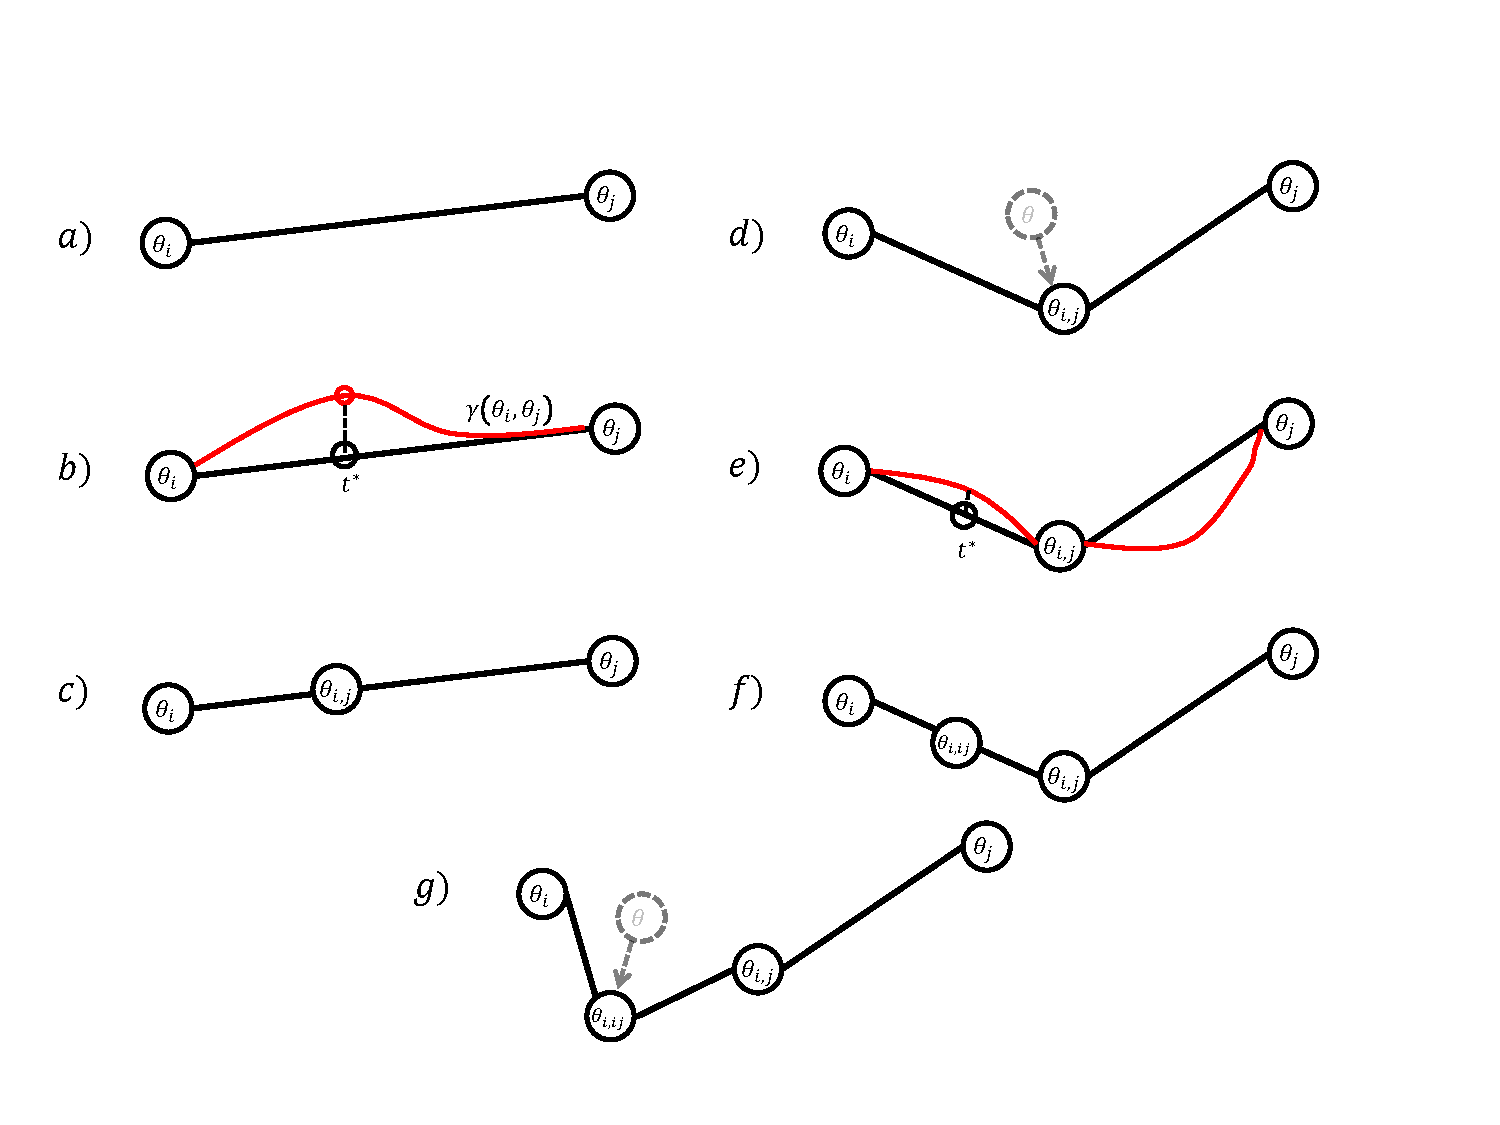
\includegraphics[width=1.0\columnwidth]{AlgorithmFigure}}
\end{center}
\caption{A cartoon of the algorithm.  $a):$ The initial two models with approximately the same loss, $L_0$. $b):$ The interpolated loss curve, in red, and its global maximum, occuring at $t=t^*$. $c):$ The interpolated model $\Theta(\theta_i, \theta_j, t^*)$ is added and labeled $\theta_{i,j}$.  $d):$ Stochastic gradient descent is performed on the interpolated model until its loss is below $\alpha L_0$. $e):$ New interpolated loss curves are calculated between the models, pairwise on a chain.  $f):$ As in step $c)$, a new model is inserted at the maxima of the interpolated loss curve between $\theta_i$ and $\theta_{i,j}$.  $g):$  As in step $d)$, gradient descent is performed until the model has low enough loss.}
\label{fig:AlgorithmFigure}
\end{figure}
 
  
  \subsection{Failure Conditions and Practicalities}
  \label{sec:Fail}
  
  While the algorithm presented will faithfully certify two models are connected if the algorithm converges, it is worth emphasizing that the algorithm does not guarantee that two models are disconnected if the algorithm fails to converge.  In general, the problem of determining if two models are connected can be made arbitrarily difficult by choice of a particularly pathological geometry for the loss function, so we are constrained to heuristic arguments for determining when to stop running the algorithm.  Thankfully, in practice, loss function geometries for problems of interest are not intractably difficult to explore.  We comment more on diagnosing disconnections more carefully in section SYMMETRYDISCONNECT.
  
  Further, if the $\rm{\mathbf{MaxError}}$ exceeds $L_0$ for every new recursive branch as the algorithm progresses, the worst case runtime scales as $O(\rm{exp}(\rm{\mathbf{Depth}}))$.  Empirically, we find that the number of new models added at each depth does grow, but eventually saturates, and falls for a wide variety of models and architectures, so that the typical runtime is closer to $O(\rm{poly}(\rm{\mathbf{Depth}}))$---at least up until a critical value of $L_0$.  We comment more on this in section NUMERICALDISCUSSION.
  
  Finally, we find that training $\Phi_3$ to $\alpha L_0$ for $\alpha < 1$ in line $8$ of the algorithm tends to aid convergence without noticeably impacting our numerics.
 

 
 %%%%%%%%%%%%%%%%%%%%%%
\section{Numerical Experiments}
\label{sec:NumExp}

For our numerical experiments, we aimed to extract qualitative features of both small, toy networks, as well as of larger workhorse networks suitable for use on real world tasks (e.g. MNIST).  At its core, the maximum interpolated error (i.e., \eqref{eq:minmaxerror}) is a measure of problem nonconvexity---or, more precisely, of the nonconvexity of the loss surface of a given architecture on a particular learning problem.


\subsection{Polynomial Regression}
\label{sec:PolyFuncs}
%%%%%%%%%%%%%%%%%%%%%%

 Polynomial function regression is a task for which small neural networks can achieve extremely high accuracy.  For our numerical experiments, we studied a 1-4-4-1 fully connected multilayer perceptron style architecture with RELU activation and RMSProp optimization.  For ease-of-analysis, we restricted the family of polynomials to be strictly contained in the interval $x\in[0,1]$ and $f(x)\in[0,1]$.
 
 Discussion of different Loss functions
 
 etc.


%%%%%%%%%%%%%%%%%%%%%%
\subsection{Convolutional Neural Networks}
\label{sec:CNN}
%%%%%%%%%%%%%%%%%%%%%%



%Exploitation
\begin{figure}
\label{figurelength}
\centering
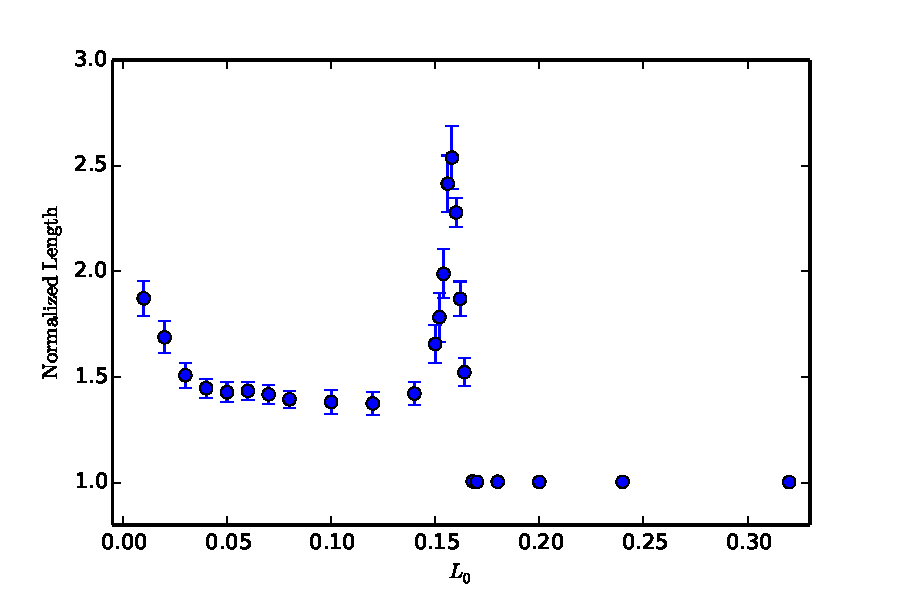
\includegraphics[width=.4\textwidth]{Plots/normlengthcubics}
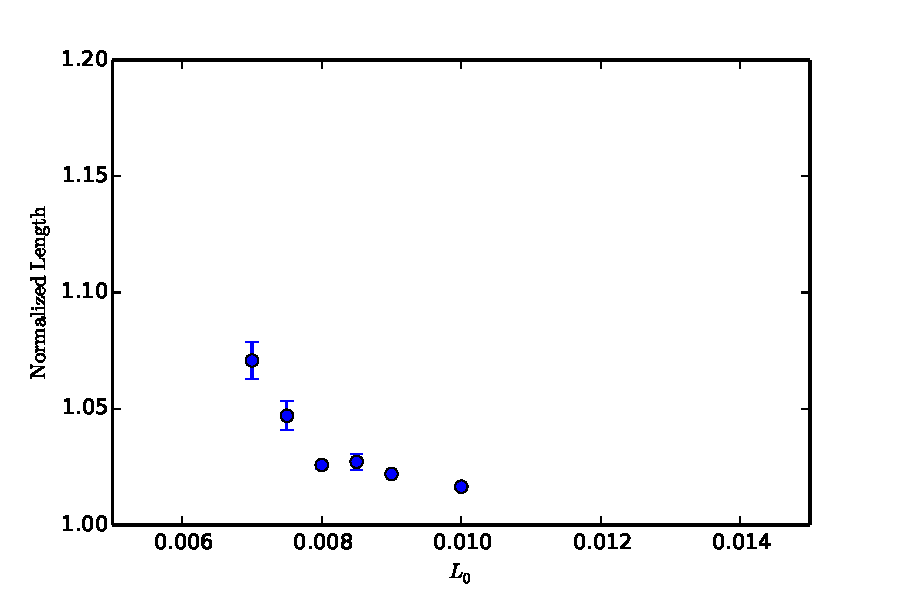
\includegraphics[width=.4\textwidth]{Plots/normlengthMNIST}
\caption{Normalized geodesic length as a function of the energy level for two different models. Left: a ``low-dimensional" neural network 
attempting to fit a cubic polynomial. Right: a convolutional neural network on MNIST. Whereas the cubic fitting displays a heavily non-convex structure 
at mid-energy values, the MNIST example qualitatively behaves as a convex loss, in which geodesics approach straight lines.}
\end{figure}


%%%%%%%%%%%%%%%%%%%%%%
%%%%%%%%%%%%%%%%%%%%%%
\section{Discussion}
\label{sec:Discussion}
%%%%%%%%%%%%%%%%%%%%%%
\begin{itemize}
\item Future: Generalization Error Question. 

\end{itemize}


\subsubsection*{Acknowledgments}

Use unnumbered third level headings for the acknowledgments. All
acknowledgments, including those to funding agencies, go at the end of the paper.

\appendix

\section{Constrained Dynamic String Sampling}
  \label{sec:ConstrainedAlg}
  
  While the algorithm presented in Sec. \ref{sec:GreedyAlg} is fast for sufficiently smooth families of loss surfaces with few saddle points, here we present a slightly modified version which, while slower, provides more control over the convergence of the string.  Instead of training intermediate models via full SGD to a desired accuracy, intermediate models will be subject to a constraint that ensures they are ``close'' to the neighboring models on the string.  Specifically, intermediate models will be constrained to the unique hyperplane in weightspace equidistant from its two neighbors.  This is similar to a sort of ``$L_1$ regularization'' where the loss function for a given model on the string, $\theta_i$, has an additional term $\tilde{L}(\theta) = L(\theta)+\zeta(\|\theta_{i-1} - \theta_i\|+\|\theta_{i+1} + \theta_i\|)$.  The strength of the $\zeta$ regularization term controls the ``springy-ness'' of the weightstring. note: make this more precise, the hyperplane constraint is stronger than the $L_1$ constraint...$L_1$ only keeps the model in a ball close to the midpoint between the models.
  
  Because adapting DSS to use this constraint is straightforward, here we will describe an alternative ``breadth-first'' approach wherein models are trained in parallel until convergence.  This alternative approach has the advantage that it will indicate a disconnection between two models ``sooner'' insofar as it will be clear two models cannot be connected once the loss on either of the two initial models, $\theta_1$ or $\theta_2$, is less than $\Gamma(\theta_1, \theta_2)$.  The precise geometry of the loss surface will dictate which approach to use in practice.
  
  Given two random models $\sigma_i$ and $\sigma_j$ where $|\sigma_i - \sigma_j| < \kappa$, we aim to follow the evolution of the family of models connecting $\sigma_i$ to $\sigma_j$.  Intuitively, almost every continuous path in the space of random models connecting $\sigma_i$ to $\sigma_j$ has, on average, the same (high) loss.  For simplicity, we choose to initialize the string to the linear segment interpolating between these two models.  If this entire segment is evolved via gradient descent, the segment will either evolve into a string which is entirely contained in a basin of the loss surface, or some number of points will become fixed at a higher loss.  These fixed points are difficult to detect directly, but will be indirectly detected by the persistence of a large interpolated loss between two adjacent models on the string.
  
  The algorithm proceeds as follows:
  
  (0.) Initialize model string to have two models, $\sigma_i$ and $\sigma_j$.
  
  1. Begin training all models to the desired loss, keeping the instantaneous loss of all models being trained approximately constant..
  
  2. If the pairwise interpolated loss $\gamma(\sigma_n,\sigma_{n+1})$ exceeds a tolerance $\alpha_1$, insert a new model at the maximum of the interpolated loss between these two models.  For simplicity, this tolerance is chosen to be $(1 + \alpha_1^*)$ times the instantaneous loss of all other models on the string.  
  
  3. Repeat steps (1) and (2) until all models (and interpolated errors) are below a threshold loss $L_0$, or until a chosen failure condition (see \ref{sec:Fail}).



\bibliography{iclr2017_conference}
\bibliographystyle{iclr2017_conference}

\end{document}
